% Just The Docs Front Matter
% title: Mesh Adaptation
% parent: Tutorials
% has_children: false
% has_toc: false

\subsection{Mesh Adaptation} \label{sec:using-issm-tutorials-mesh}
\subsubsection{Goals} %{{{
In this tutorial, we show how to use the different meshers of ISSM:
\begin{itemize}
	\item Learn how to use the different meshers of ISSM:
		\begin{itemize}
			\item \lstinlinebg|squaremesh| for square domains (ISMIP)
			\item \lstinlinebg|roundmesh| for round domain (EISMINT)
			\item \lstinlinebg|triangle| (from J. Shewchuk)
			\item \lstinlinebg|bamg| (adapted from F. Hecht)
		\end{itemize}
	\item Use anisotropic mesh adaptation to optimize the mesh resolution spatially
\end{itemize}
Go to \lstinlinebg|<ISSM_DIR>/examples/Mesh/| to do this tutorial.
%}}}

\subsubsection{Squaremesh}%{{{
\lstinlinebg|squaremesh| generates structured uniform meshes for rectangular domains.
\paragraph{Usage}%{{{
\begin{lstlisting}
>> md = model;
>> md = squaremesh(md, 100, 200, 15, 25);
\end{lstlisting}
\lstinlinebg|squaremesh| takes the following arguments:
\begin{enumerate}
	\item model
	\item x-length (meters)
	\item y-length (meters)
	\item number of nodes along the x axis
	\item number of nodes along the y axis
\end{enumerate}
%}}}

\paragraph{Example}%{{{
The previous command creates the mesh shown below:
\begin{lstlisting}
>> plotmodel(md, 'data', 'mesh');
\end{lstlisting}
\begin{figure}[H]
	\begin{center}
		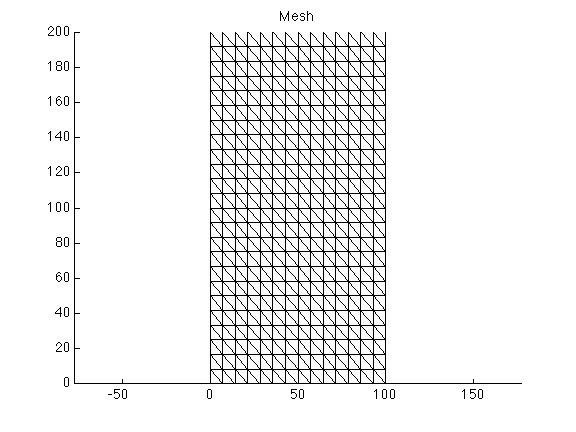
\includegraphics[width=\textwidth]{\assetsParentPath/assets/img/using-issm/tutorials/mesh/mesh1.png}
	\end{center}
\end{figure}
%}}}
%}}}
\subsubsection{Roundmesh}%{{{
\lstinlinebg|roundmesh| generates unstructured uniform meshes for circular domains.

\paragraph{Usage}%{{{
\begin{lstlisting}
>> md = roundmesh(model, 100, 10);
\end{lstlisting}
\lstinlinebg|roundmesh| takes the following arguments:
\begin{enumerate}
	\item model
	\item radius (meters)
	\item element size (meters)
\end{enumerate}
%}}}

\paragraph{Example}%{{{
The previous command creates the mesh shown below:
\begin{lstlisting}
>> plotmodel(md, 'data', 'mesh');
\end{lstlisting}
\begin{figure}[H]
	\begin{center}
		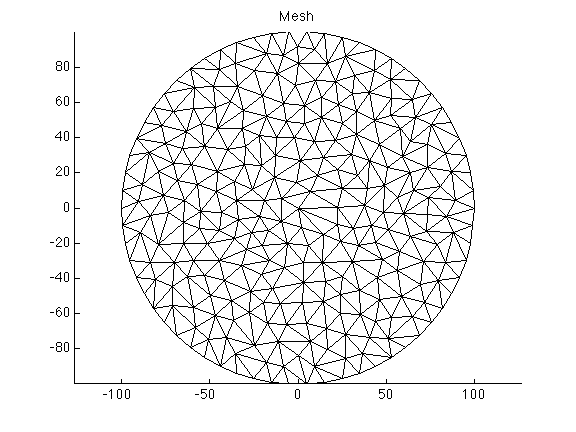
\includegraphics[width=\textwidth]{\assetsParentPath/assets/img/using-issm/tutorials/mesh/mesh2.png}
	\end{center}
\end{figure}
%}}}

\subsubsection{Triangle}%{{{
\lstinlinebg|triangle| is a very fast algorithm for mesh generation. Developed by \href{http://www.cs.cmu.edu/~quake/triangle.html}{J Shewchuk}, it generates unstructured triangular meshes.

\paragraph{Usage}%{{{
\begin{lstlisting}
>> md = triangle(model, 'Square.exp', .2);
\end{lstlisting}
\lstinlinebg|triangle| takes the following arguments:
\begin{enumerate}
	\item model
	\item ARGUS file of the domain outline (\lstinlinebg|.exp| extension, see the 
	%__@LATEX_ONLY_START@__
	\hyperref[sec:using-issm-capabilities-mesh-generation]{`Capabilities' $\rightarrow$ `Mesh Generation' section}
	%__@LATEX_ONLY_END@__
	%__@MARKDOWN_ONLY_START@__
	%<a href="../capabilities/mesh-generation" target="_top">'Capabilities' &#8594; 'Mesh Generation' page</a>
	%__@MARKDOWN_ONLY_END@__
	for more details)
	\item average element size (meters)
\end{enumerate}
The previous command creates the following mesh:
\begin{lstlisting}
>> plotmodel(md, 'data', 'mesh');
\end{lstlisting}
\begin{figure}[H]
	\begin{center}
		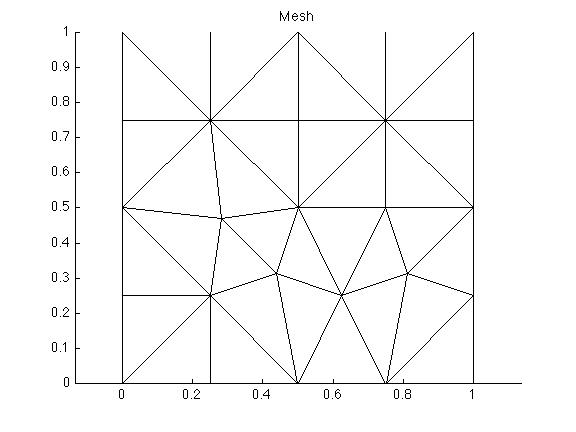
\includegraphics[width=\textwidth]{\assetsParentPath/assets/img/using-issm/tutorials/mesh/mesh3.png}
	\end{center}
\end{figure}
You can change the resolution from \lstinlinebg|0.2| to \lstinlinebg|0.05| to get a higher resolution.
%}}}

\subsubsection{Bamg}%{{{
BAMG stands for Bidimensional Anisotropic Mesh Generator. It was released in 2006 after more than 10 years of development by Frederic Hecht. It is now part of \href{http://www.freefem.org/ff++/}{FreeFEM++}. The algorithm that is available in ISSM is inspired by this software, but has been rewritten entirely.
%}}}

\paragraph{Usage}%{{{
\begin{lstlisting}
>> md = bamg(model, ...);
\end{lstlisting}
\lstinlinebg|bamg| takes as it's first argument a model, and then pairs of options
\begin{enumerate}
	\item model
	\item pairs of options (type \lstinlinebg|help bamg| to get a full list of options)
\end{enumerate}
%}}}

\paragraph{Uniform mesh}%{{{
To create a non-uniform mesh, use the following options:
\begin{enumerate}
	\item \lstinlinebg|'domain'| followed by the domain name
	\item \lstinlinebg|'hmax'| followed by the size (meters) of each triangle
\end{enumerate}
\begin{lstlisting}
>> md = bamg(model, 'domain', 'Square.exp', 'hmax', .05);
\end{lstlisting}
The previous command will create the following mesh (use \lstinlinebg|plotmodel(md, 'data', 'mesh')| to visualize the mesh):
\begin{figure}[H]
	\begin{center}
		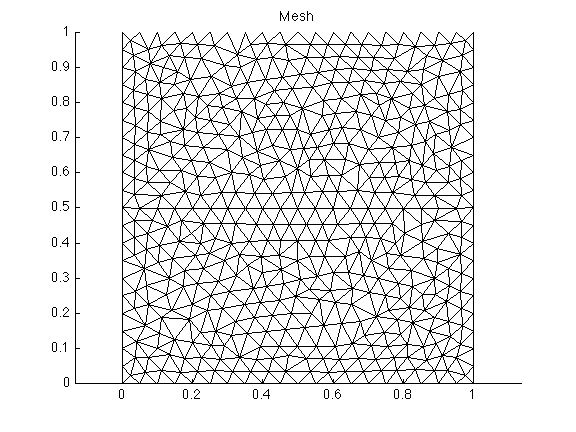
\includegraphics[width=\textwidth]{\assetsParentPath/assets/img/using-issm/tutorials/mesh/mesh4.png}
	\end{center}
\end{figure}
Note that the nodes are not as randomly distributed as \lstinlinebg|triangle|. The strength of BAMG is not for uniform meshes but for automatic mesh adaptation based on a metric.
%}}}

\paragraph{Non-Uniform mesh}%{{{
To create a non-uniform mesh, use the following options:
\begin{enumerate}
	\item \lstinlinebg|'domain'| followed by the domain name
	\item \lstinlinebg|'hvertices'| followed by the element size for each vertex of the domain outline
\end{enumerate}
In our example, \lstinlinebg|Square.exp| has 4 vertices. If we want a resolution of 0.2, except in the vicinity of the third node, we use the following commands:
\begin{lstlisting}
>> md = model;
>> hvertices = [0.2; 0.2; 0.005; 0.2];
>> md = bamg(md, 'domain', 'Square.exp', 'hvertices', hvertices);
\end{lstlisting}
Use the \lstinlinebg|plotmodel(md, 'data', 'mesh')| command to visualize the newly defined mesh:
\begin{figure}[H]
	\begin{center}
		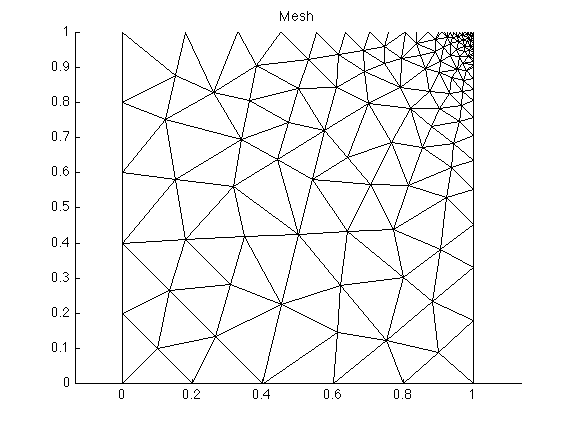
\includegraphics[width=\textwidth]{\assetsParentPath/assets/img/using-issm/tutorials/mesh/mesh5.png}
	\end{center}
\end{figure}
%}}}

\paragraph{Mesh adaptation}%{{{
We can use observations to generate a mesh that is adapted to the solution we are trying to model. Given a solution field, \lstinlinebg|bamg| will calculate a metric based on the field's Hessian matrix (second derivative) to generate an anisotropic mesh that minimize the interpolation error (assuming that linear finite elements are used).

For a first example, we are going to use the observations given by the function \lstinlinebg|shock.m|. It generates a discontinuity that requires the mesh to be highly refined along a circle.
\begin{figure}[H]
	\begin{center}
		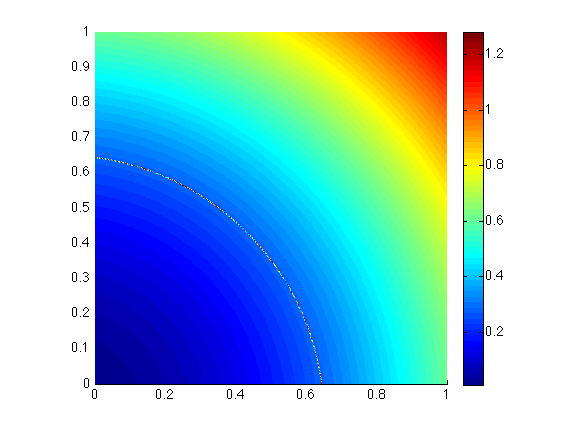
\includegraphics[width=\textwidth]{\assetsParentPath/assets/img/using-issm/tutorials/mesh/shock0.png}
	\end{center}
\end{figure}
First, we generate a simple uniform mesh. We interpolate the observations on the vertices of this mesh:
\begin{lstlisting}
>> md = bamg(model, 'domain', 'Square.exp', 'hmax', .05);
>> vel = shock(md.mesh.x, md.mesh.y);
>> plotmodel(md, 'data', vel, 'edgecolor', 'w');
\end{lstlisting}
\begin{figure}[H]
	\begin{center}
		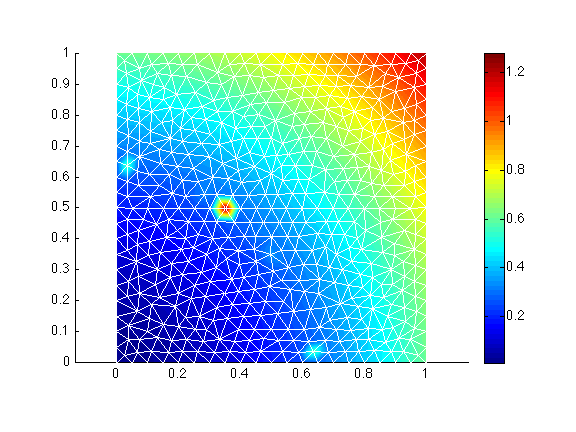
\includegraphics[width=\textwidth]{\assetsParentPath/assets/img/using-issm/tutorials/mesh/shock1.png}
	\end{center}
\end{figure}
With a simple uniform mesh, the discontinuity is not captured. It is best to start with a finer mesh, which captures the discontinuity rather well, and interpolate the observations on this finer mesh to adapt the mesh anisotropically.
\begin{lstlisting}
>> md = bamg(model, 'domain', 'Square.exp', 'hmax', .005);
>> vel = shock(md.mesh.x, md.mesh.y);
\end{lstlisting}
Now, we call \lstinlinebg|bamg| a second time to adapt the mesh according the \lstinlinebg|vel|. We do not reinitialize \lstinlinebg|md| and call \lstinlinebg|bamg| again without specifying the \lstinlinebg|'domain'|, as a first mesh already exists in the model. We provide the following options:
\begin{enumerate}
	\item \lstinlinebg|'field'| followed by \lstinlinebg|vel|, the field we want to adapt the mesh to
	\item \lstinlinebg|'err'| the allowed interpolation error (Here, the field must be captured within 0.05)
	\item \lstinlinebg|'hmin'| minimum edge length
	\item \lstinlinebg|'hmax'| maximum edge length
\end{enumerate}
\begin{lstlisting}
>> md = bamg(md, 'field', vel, 'err', 0.05, 'hmin', 0.005, 'hmax', 0.3);
>> vel = shock(md.mesh.x, md.mesh.y);
>> plotmodel(md, 'data', vel, 'edgecolor', 'w');
\end{lstlisting}
\begin{figure}[H]
	\begin{center}
		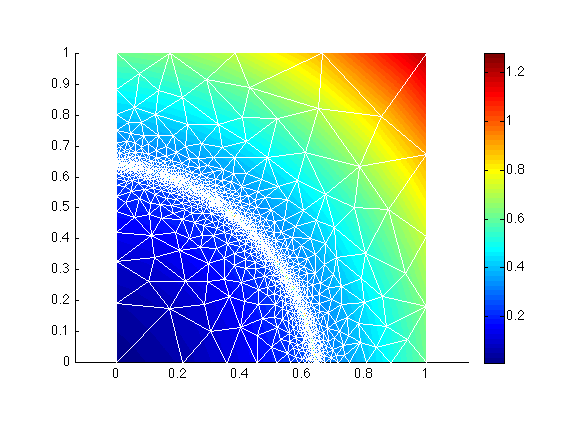
\includegraphics[width=\textwidth]{\assetsParentPath/assets/img/using-issm/tutorials/mesh/shock2.png}
	\end{center}
\end{figure}
You can change the option \lstinlinebg|'err'| to 0.03, to see the effect of \lstinlinebg|'err'|. The ratio between two consecutive edges can be controlled by the option \lstinlinebg|'gradation'|.
\begin{lstlisting}
>> md = bamg(model, 'domain', 'Square.exp', 'hmax', .005);
>> vel = shock(md.mesh.x, md.mesh.y);
>> md = bamg(md, 'field', vel, 'err', 0.03, 'hmin', 0.005, 'hmax', 0.3, 'gradation', 3);
>> vel = shock(md.mesh.x, md.mesh.y);
>> plotmodel(md, 'data', vel, 'edgecolor', 'w');
\end{lstlisting}
\begin{figure}[H]
	\begin{center}
		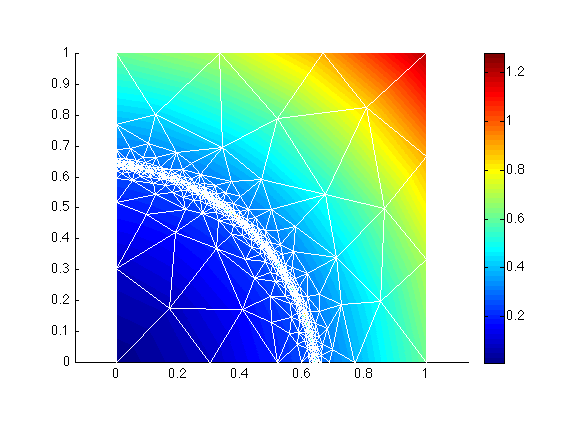
\includegraphics[width=\textwidth]{\assetsParentPath/assets/img/using-issm/tutorials/mesh/shock3.png}
	\end{center}
\end{figure}
We can also force the triangles to be equilateral by using the \lstinlinebg|'anisomax'| option, which specifies the maximum level of anisotropy (between 0 and 1, 1 being fully isotropic).
\begin{lstlisting}
>> md = bamg(model, 'domain', 'Square.exp', 'hmax', .005);
>> vel = shock(md.mesh.x, md.mesh.y);
>> md = bamg(md, 'field', vel, 'err', 0.03, 'hmin', 0.005, 'hmax', 0.3, 'gradation', 1.3, 'anisomax', 1);
>> vel = shock(md.mesh.x, md.mesh.y);
>> plotmodel(md, 'data', vel, 'edgecolor', 'w');
\end{lstlisting}
\begin{figure}[H]
	\begin{center}
		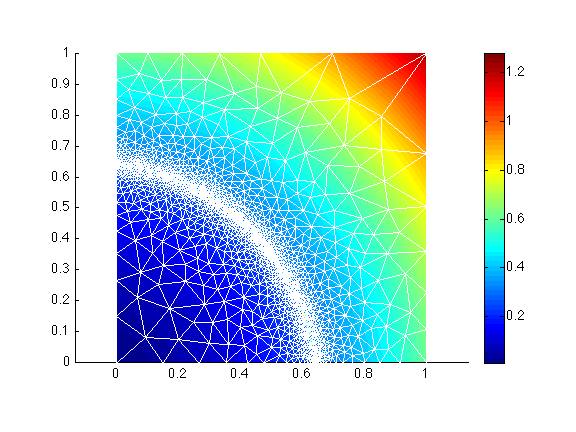
\includegraphics[width=\textwidth]{\assetsParentPath/assets/img/using-issm/tutorials/mesh/shock4.png}
	\end{center}
\end{figure}
You can also try to refine a mesh using the function \lstinlinebg|circles.m|, which is provided in the same directory.
%}}}

\paragraph{Mesh refinement in a specific region}%{{{
It is sometimes necessary to specify a mesh resolution for an area of interest. We will use the same example as before. The first step consists of creating an ARGUS file that defines the region where we want to refine the mesh.

We first plot \lstinlinebg|vel| and we call the function \lstinlinebg|exptool| to create a file \lstinlinebg|refinement.exp| that defines this region. Select \lstinlinebg|add a contour (closed)|. Draw a contour over a given region, hit enter when you are done, and then select quit. You should now see the \lstinlinebg|refinement.exp| file in the current directory.
\begin{lstlisting}
>> plotmodel(md, 'data', vel, 'edgecolor', 'w');
>> exptool('refinement.exp')
\end{lstlisting}
\begin{figure}[H]
	\begin{center}
		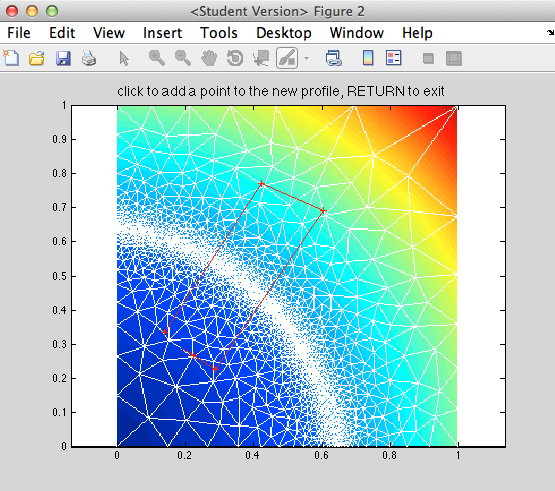
\includegraphics[width=\textwidth]{\assetsParentPath/assets/img/using-issm/tutorials/mesh/exptool.png}
	\end{center}
\end{figure}

Now, we are going to create a vector that specifies, for each vertex of the existing mesh, the resolution of the adapted mesh. We use \lstinlinebg|NaN| for the vertices we do not want to change. So in this example, this will be a vector of \lstinlinebg|NaN|, except for the vertices in \lstinlinebg|refinement.exp|, where we want a resolution of 0.02:
\begin{lstlisting}
>> h = NaN * ones(md.mesh.numberofvertices, 1);
>> in = ContourToNodes(md.mesh.x, md.mesh.y, 'refinement.exp', 1);
>> h(find(in)) = 0.02;
>> plotmodel(md, 'data', in, 'edgecolor', 'w');
\end{lstlisting}
You will see that all the vertices that are in \lstinlinebg|refinement.exp| have a value of 1 (they are inside the contour), and the others are 0.
\begin{figure}[H]
	\begin{center}
		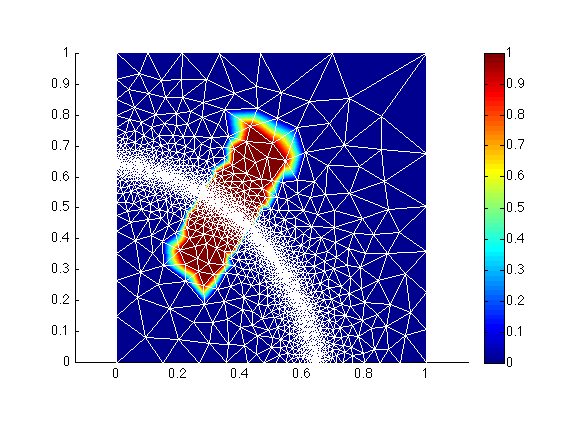
\includegraphics[width=\textwidth]{\assetsParentPath/assets/img/using-issm/tutorials/mesh/refine1.png}
	\end{center}
\end{figure}

Now, we call \lstinlinebg|bamg| a third time, with the specified resolution for the vertices that are in \lstinlinebg|refinement.exp|:
\begin{lstlisting}
>> vel = shock(md.mesh.x, md.mesh.y);
>> md = bamg(md, 'field', vel, 'err', 0.03, 'hmin', 0.005, 'hmax', 0.3, 'hVertices', h);
>> vel = shock(md.mesh.x, md.mesh.y);
>> plotmodel(md, 'data', vel, 'edgecolor', 'w');
\end{lstlisting}
\begin{figure}[H]
	\begin{center}
		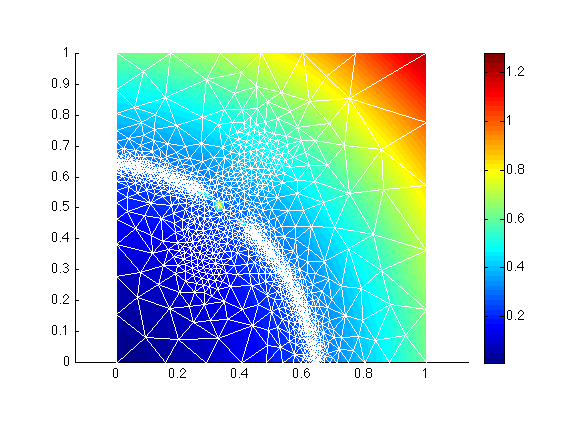
\includegraphics[width=\textwidth]{\assetsParentPath/assets/img/using-issm/tutorials/mesh/refine2.png}
	\end{center}
\end{figure}
%}}}

\paragraph{Another example}%{{{
If you would like to try another example, you can use the function \lstinlinebg|circles.m| instead of
\lstinlinebg|shock.m|. It is also a 1x1 square but with a pattern that includes five circles.
%}}}

\clearpage % Make sure all figures are placed before next section
